%!TEX root =  main.tex
\section{Background}

\fp{In this section, we should define SMR, S-SMR and DS-SMR!}

State machine replication is a fundamental approach to implementing a fault-tolerant service by replicating servers and coordinating the execution of client commands against server replicas~\cite{Lam78,Sch90}. 
State machine replication ensures strong consistency (i.e., linearizability~\cite{Attiya04}) by coordinating the execution of commands in the different replicas: Every replica has a full copy of the service state $\vvm = \{v_1, ..., v_m\}$ and executes commands submitted by the clients in the same order. A command is a program consisting of a sequence of operations, which can be of three types: $read(v)$, $write(v, val)$, or a deterministic computation.

\subsection{Scaling state machine replication}
By starting in the same initial state and executing the same sequence of deterministic commands, servers make the same state changes and produce the same reply for each command. To guarantee that servers deliver the same sequence of commands, SMR can be implemented with atomic broadcast: commands are atomically broadcast to all servers, and all correct servers deliver and execute the same sequence of commands \cite{BJ87b,DSU04}.

Despite its simple execution model, classical SMR does not scale: adding resources (e.g., replicas) will not translate into sustainable improvements in throughput. This happens for a couple reasons. First, the underlying communication protocol needed to ensure ordered message delivery may not scale itself (i.e., a communication bottleneck). Second, every command must be executed sequentially by each replica (i.e., an execution bottleneck).

Several approaches have been proposed to address SMR's scalability limitations. To cope with communication overhead, some proposals have suggested to spread the load of ordering commands among multiple processes (e.g., \cite{Moraru:2013gw,Mencius,Marandi:2012hb}), as opposed to dedicating a single process to determine the order of commands (e.g., \cite{Lamport:1998ea}).%\fxnote[draft]{remove inapplicable reference}

Two directions of research have been suggested to overcome execution bottlenecks. One approach (scaling up) is to take advantage of multiple cores to execute commands concurrently without sacrificing consistency \cite{Kapritsos:2012um,Marandi:2014bj,Kotla:2004ep,Guo:2014jp}. Another approach (scaling out) is to partition the service's state and replicate each partition (e.g., \cite{Glendenning:2011kj,Marandi:2011dj}). In the following section, we review Scalable State Machine Replication (\ssmr), a proposal in the second category.

\subsection{Scalable State Machine Replication}
\label{sec:ssmr}

In S-SMR~\cite{bezerra2014ssmr}, the service state \vvt\ is composed of $k$ partitions, in set $\Psi = \{\ppm_1, ..., \ppm_k\}$. Server group $\ssm_i$ is assigned to partition $\ppm_i$. For brevity, we say that server $s$ belongs to $\ppm_i$ meaning that $s \in \ssm_i$, and say ``multicast to $\ppm_i$" meaning ``multicast to server group $\ssm_i$".
S-SMR relies on an \emph{oracle}, which tells which partitions are accessed by each command.%
\footnote{The oracle returns a set with the partitions accessed by the command, but this set does not need to be minimal; it may contain all partitions in the worst case, when the partitions accessed by the command cannot be determined before the command is executed.}

To execute a command, the client multicasts the command to the appropriate partitions, as determined by the oracle.
Commands that access a single partition are executed as in classical SMR: replicas of the concerned partition agree on the execution order and each replica executes the command independently.
In the case of a multi-partition command, replicas of the involved partitions deliver the command and then may need to exchange state in order to execute the command since some partitions may not have all the values read in the command.
This mechanism allows commands to execute seamlessly despite the partitioned state.

%\begin{algorithm}[t!]
\small

\begin{distribalgo}[1]

\vspace{1mm}

\INDENT{\emph{Initialization:}}
    \STATE $\forall C \in $ \kk $ : rcvd\_signals(C) \leftarrow \emptyset$
    \STATE $\forall C \in $ \kk $ : rcvd\_variables(C) \leftarrow \emptyset$
\ENDINDENT

\vspace{1.25mm}
\INDENT{\emph{Command $C$ is submitted by a client as follows:}}
    \STATE $C.dests \leftarrow oracle(C)$ \label{algline:oracle} 
	\STATE \amcast$(C.dests, C)$ \label{algline:climcast}
	\STATE wait for reply
\ENDINDENT

\vspace{1.25mm}
\INDENT{\emph{Server $s$ of partition \pp\ executes command $C$ as follows:}}
	\INDENT{\textbf{when} \amdel$(C)$}
	    \STATE $others \leftarrow C.dests \setminus \{\ppm{}\}$
	    \STATE \rmcast$(others, signal(C))$ \label{algline:mcastsignals}
		\FOR{each operation $op$ in $C$}
			\IF{$op$ is $read(v)$}
			    \IF{$v \in \ppm$}
			        \STATE \rmcast$(others, \langle v, C.id \rangle)$ \label{algline:multicastv}
			    \ELSE
			        \STATE \textbf{wait until} $v \in rcvd\_variables(C)$ \label{algline:waitvariable}
			        \STATE update $v$ with the value in $rcvd\_variables(C)$
			    \ENDIF
			\ENDIF
			\STATE execute $op$ \label{algline:executeopck}
		\ENDFOR
		\STATE \textbf{wait until} $rcvd\_signals(C) = others$ \label{algline:waitsignals}
		\STATE send reply to client \label{algline:sendreply}
	\ENDINDENT
	
	\vspace{1.25mm}
	\INDENT{\textbf{when} \rmdel$(signal(C))$ from partition $\ppm'$}
	    \STATE $rcvd\_signals(C) \leftarrow rcvd\_signals(C) \cup \{\ppm'\}$
	\ENDINDENT

	\vspace{1.25mm}
	\INDENT{\textbf{when} \rmdel$(\langle v, C.id \rangle)$}
	    \STATE $rcvd\_variables(C) \leftarrow rcvd\_variables(C) \cup \{v\}$
	\ENDINDENT
			
\ENDINDENT

\vspace{1.7mm}

\textbf{Algorithm variables:}

\vspace{1.25mm}

\kk: the set of all possible commands

\vspace{1mm}

$C.id$: unique identifier of command $C$

\vspace{1mm}

$oracle(C)$: function that returns a superset of the partitions accessed by $C$

\vspace{1mm}

$C.dests$: set of partitions to which $C$ is multicast

\vspace{1mm}

$others$: set of all partitions, other than \pp{}, where $C$ is executed.

\vspace{1mm}

$signal(C)$: signal exchanged to ensure linearizability

\vspace{1mm}

$rcvd\_signals(C)$: set of all partitions that already signaled \pp\ regarding $C$

\vspace{1mm}

$rcvd\_variables(C)$: set of all variables received from other partitions in order to execute $C$

\caption{Scalable State Machine Replication (\ssmr)}
\label{alg:ssmr}
\end{distribalgo}
\end{algorithm}

%\begin{figure*}
%\begin{minipage}[b]{1\linewidth} % A minipage that covers the whole width of the page
%\centering
%      \includegraphics[width=1.0\linewidth]{figures/move_case_1}
%\end{minipage}
%\caption{Consulting the oracle and issuing a command are done in multiple calls to \amcast{}. White boxes represent actions of the client proxy.}
%\label{fig:move_case_1}
%\end{figure*}

Algorithm~\ref{alg:ssmr} shows precisely how S-SMR operates. When a server $s$ of partition $\ppm$, while executing a command $C$, reaches a $read(v)$ operation, there are two possibilities:
either $v$ belongs to the local partition $\ppm$,
or it is part of a remote partition $\ppm'$. 
If $v$ is local, $s$ will retrieve its value and send it to the servers of other partitions concerned by $C$;
if $v$ is remote, $s$ will wait until its value is received from a server of $\ppm'$. 
A $write(v, val)$ operation does not depend on the previous value of $v$, not requiring communication between partitions, even if $v$ is not assigned to the partition of the server executing $C$.
To ensure linearizability, all partitions involved in the execution of a multi-partition command $C$ must coordinate before a reply can be sent to the client.
%To understand why, consider the non-linearizable execution shown in Figure~\ref{fig:whysignals}~(a).
%This execution is not linearizable because the only equivalent sequential execution requires $C_y$ to precede $C_{xy}$ and $C_{xy}$ to precede $C_x$, thus $C_y$ would precede $C_x$.
%Although this execution does not violate atomic order, it contradicts real-time ordering, in which $C_x$ precedes $C_y$.
In \ssmr{}, partitions exchange signals while executing multi-partition commands~\cite{bezerra2014ssmr}.
This guarantees linearizability, at the cost of synchronizing partitions.


S-SMR improves on classical SMR by allowing replicated systems to scale, while ensuring linearizability. 
Under workloads with multi-partition commands, however, it has limited performance, in terms of latency and throughput scalability. 
Such decreased performance when executing multi-partition commands is due to
partitions (i) exchanging state variables
and (ii) synchronizing by exchanging signals.
\ssmr\ performs better as the number of multi-partition commands decreases.

One way to reduce the number of multi-partition commands is by dynamically changing the partitioning, putting variables that are usually accessed together in the same partition.
However, the partitioning oracle of \ssmr\ relies on a static mapping of variables to partitions.
One advantage of this implementation is that all clients and servers can have their own local oracle, which always returns a correct set of partitions for every query.
Such a static mapping has the major limitation of not allowing the service to dynamically adapt to different access patterns.

\subsection{Graph partitioning}
%What is graph partitioning?
Graph partitioning is an important subproblem of any system that aims parallelization and thus scalability, a bad partitioning can undermine all effort done in other parts of the system, so having the data well and evenly distributed is fundamental.

%Need to relate the objects to the graph so it makes sense to use already functioning graph partitioning algorithms.

%Definition of Graph partitioning
Given a graph $G = (V, E)$, and a number of partitions $k$, a partition $p_i$ with $1 \leq i \leq k$ is a subset of $V$ such that $\bigcup p_i = V$ and $\bigcap p_i = \emptyset$.

%What is a good partitioning? Our definition:
We define a good partitioning as one that minimize the cross-edges among partitions while maintaining each partition balanced, more formally, let $C(P)$ be a set of edges connecting a vertex in $P$ with a vertex in $V - P$, ideally $\frac{\sum_{i=1}^{k}|C(p_i)|}{|E|} = 0$ and $\frac{max_{1 \leq i \leq k}(|p_i|)}{avg_{1 \leq i \leq k}(|p_i|)} = 1$
